\section{Theory}
\subsection{Recurrent Neural Network (RNN)} RNN is a variant of the Artificial Neural Network (ANN) where the nodes in the hidden layer are connected in such a way that these nodes store data from the previous time step which help in utilizing the connection between the input sequences \cite{DBLP:journals/corr/abs-1808-03314}.

\subsection{Long-Short Term Memory Networks (LSTM)} LSTM is a type of RNN where the network remembers long sequence of input and tries to find the important sequences to remember in the whole input. This variant works better than RNN because it solves the problem of vanishing gradient where the old data is forgotten completely based on how far it is from the current instance of input \cite{DBLP:journals/corr/abs-1808-03314}. It does not consist of just one activation function to the input but rather an input data inside these neurons goes through a series of gates. Two major checkpoints inside LSTM unit is the forget and the write gate. Write gate helps the RNN decide which part of the information to be retained or written. Forget gate helps RNN forget the non-important information and scrap it and produce a filter through which only the most important information can pass through, which in turn reduces the load of long dependencies and helps remember the previous context.

\subsection{Bi-Directional LSTM} Bidirectional LSTMs are an extension of traditional LSTMs that can improve model performance on sequence classification problems \cite{Schuster97bidirectionalrecurrent}. The principle of Bidirectional LSTMs is to connect two hidden layers running in opposite directions, one for positive time direction (forward states), and another for negative time direction (backward states) to a single output. In our case, \say{time} refers to each word in the input sequence. The advantage bidirectional LSTM offers over traditional LSTM is that the neural network has access to information from the past and the future thus helping it gain context from both directions without the use of more sophisticated LSTM layers.
\begin{figure}[h]
	\begin{center}
		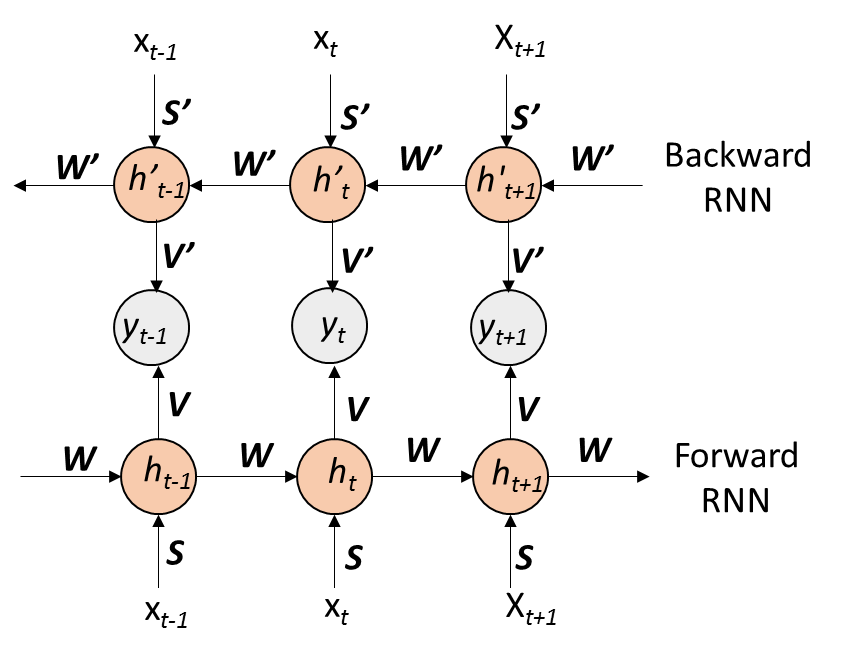
\includegraphics[width=150pt]{figures/bidirectional.png}
		\captionsource{Working of Bi-directional LSTM}{https://subscription.packtpub.com/book/big\_data\_and\_business\_intelligence\\
		/9781787121089/6/ch06lvl1sec69/setting-up-a-bidirectional-rnn-model}
		\label{fig:bidilstm}
	\end{center}
\end{figure}\newline
In the picture, \say{w} is the weights that are updated from taking the sequence in its right order (\say{s}) and \say{w'} are the weights that are updated from the taking the sequence in reverse (\say{s'}). \say{h} and \say{h'} are the hidden nodes for forward and backward sequences respectively and \say{x} and \say{y} are input and output nodes.
From the picture above, the forward RNN is responsible for handling the input data in the usual direction and backward RNN is responsible for the reverse sequence of the input data. Both, the forward and backward LSTM combine to give output for that particular time-step (t-1, t, t+1) or word-step(our case).
\subsection{Lemmatization}
Lemmatization is the process of reducing the words to their root words i.e. \say{asked}, \say{asking} will be reduced to \say{ask}. This mostly helps in reducing the number of unique words but keeping the intent same \cite{Manning:2008:IIR:1394399}. This can be done using the NLTK package which is readily available in python \cite{Loper:2002:NNL:1118108.1118117}.
\subsection{STOP Words}
While working with textual data, there will always be words that occur most frequently but do not contribute significantly to the essence of the text \cite{Manning:2008:IIR:1394399}. Such words are known as STOP words. Removing such words helps in reducing the time spent on indexing the words and helps in concentrating on words that actually contribute to the meaning. This can be done using the NLTK package which is readily available in python. \cite{Loper:2002:NNL:1118108.1118117}
\subsection{Contractions}
 Contractions are shortened words mostly present in spoken vocabulary and ultimately adopted to written. In English, an example of contraction of phrase \say{I have} would be \say{I’ve}. We expand such contractions so that we have some sort of standardization of text \cite{Sarkar:2016:TAP:3086768}. A typical way of dealing with contractions is to make a table of all known contractions and expand all the current contractions we found in the text corpus via the given table. 
 \subsection{Word Embeddings}
 Word embeddings is a natural language modelling technique that turns text into vector representations(made of numbers) of a word. This transformation is necessary because machine learning algorithms require their input to be numbers since the models don't work on strings of plain text. Embeddings map words or phrases from a vocabulary to a corresponding vector of real numbers. Word embeddings are usually used for following properties:
 \begin{itemize}
     \item Dimensionality Reduction: Usually, when dealing with large corpus of textual data, the dimensionality of vectors formed is very large and word embedding aims to create a vector representation of them in a much lower dimensional space \cite{pennington2014glove}. This is achieved effectively by combining PCA based dimensionality reduction with a post-processing algorithm, to construct word embeddings of lower dimensions.\cite{DBLP:journals/corr/abs-1708-03629}
     \item Contextual Similarity: For a language model to be able to predict the meaning of text, it needs to be aware of the contextual similarity of words.\cite{DBLP:journals/corr/MikolovSCCD13}
     A measure of similarity of words can be achieved by taking cosine of the word vectors. The standard comparison metric is cosine similarity, which is equivalent to dot product if the vectors are normalized. Other metrics include Euclidean distance, the less-known Tanimoto similarity, which is similar to cosine similarity but with a different normalization factor.\cite{Thesis}
 \end{itemize}
 \subsection{Class Imbalance}
 Class imbalance refers to the phenomenon where some classes (labels) of a dataset have more samples than others. This is a problem because the machine learning algorithms will tend to focus on the classification of the samples that are over represented while ignoring or misclassifying the underrepresented samples. In our dataset, we have only 80810 samples of insincere questions and 1225312 samples of sincere questions. The classifier will tend to classify insincere questions as sincere ones. There are several methods to overcome this problem:
 \begin{itemize}
     \item Undersampling- Under sampling is a method where we try to extract samples from the main dataset, in a sense to balance the dataset where the no. of target classes have approximately equal no of samples. We remove some of the majority class samples from the dataset in order to balance the majority and minority class samples, so it has less effect on the machine learning algorithm. However, we could risk discarding useful information as some of the majority class instances might be more representative and we run a risk of removing these instances. \cite{Liu:2009:ITC:1453254.1453338}
     \item Oversampling- Instead of removing samples of majority classes, we add more samples of the minority class by replication, so it has more effect on the machine learning algorithm \cite{Liu:2009:ITC:1453254.1453338}. However, just duplicating the minority classes could lead the classifier to overfit a few examples.
     \item SMOTE - An over-sampling approach in which the minority class is over-sampled by creating \say{synthetic} examples rather than by over-sampling with replication \cite{DBLP:journals/corr/abs-1106-1813}. SMOTE iterates over the existing, real minority class instances. At each iteration, it chooses one of the K closest minority class neighbours and synthesizes a new minority instance somewhere between the minority instance and that neighbour. Depending upon the amount of over-sampling required, neighbors from the k nearest neighbors are randomly chosen.
 \end{itemize}
 
 \subsection{Performance Measures}
 Accuracy is not the metric to use when working with an imbalanced dataset. It is very misleading. There are other metrics that give a better story about the performance of the model when working with imbalanced classes such as: Precision, Recall and F1 Score.
 \begin{itemize}
     \item Precision: Precision is the ratio of correctly predicted positive observations to the total predicted positive observations. 
     \item Recall: Recall is the ratio of correctly predicted positive observations to the all observations in sample test data.
     \item F1-Score: F1 Score is the weighted average of Precision and Recall. Therefore, this score takes both false positives and false negatives into account. It is used as a measure between the precision and the recall and gives a sense of how balanced the model is in predicting the right labels in whole of the sample.
 \end{itemize}
 The formula for F1-score is given by $F_{1}=2 \times \frac{\text{precision} \times \text{recall}}{\text{precision} + \text{recall}}$
 \newline
 Intuitively F1 score is not as easy to understand as accuracy, but it is usually more useful than accuracy, especially if you have an uneven class distribution.